\documentclass[11pt]{article}
\usepackage{geometry}
% Additional packages
\usepackage[utf8]{inputenc}
\usepackage{pdfpages}
% Boxed floats
\usepackage{float}
%\floatstyle{boxed} 
%\restylefloat{figure}
%
% MATLAB integration
\usepackage{listings}
\usepackage{color}
\usepackage{textcomp}
\definecolor{listinggray}{gray}{0.9}
\definecolor{lbcolor}{rgb}{0.98,0.98,0.98}
\lstset{
	backgroundcolor=\color{lbcolor},
	tabsize=4,
	language=Matlab,
	basicstyle=\scriptsize,
	upquote=true,
	aboveskip={1.5\baselineskip},
	columns=fixed,
	showstringspaces=false,
	extendedchars=true,
	breaklines=true,
	%prebreak = \raisebox{0ex}[0ex][0ex]{\ensuremath{\hookleftarrow}},
	frame=single,
	showtabs=false,
	showspaces=false,
	showstringspaces=false,
	identifierstyle=\ttfamily,
	keywordstyle=\color[rgb]{0,0,1},
	commentstyle=\color[rgb]{0.133,0.545,0.133},
	stringstyle=\color[rgb]{0.627,0.126,0.941},
}
%
%

\geometry{letterpaper}                   

\usepackage{graphicx}
\usepackage{amssymb}
\usepackage{epstopdf}
\usepackage{natbib}
\usepackage{amssymb, amsmath}
\DeclareGraphicsRule{.tif}{png}{.png}{`convert #1 `dirname #1`/`basename #1 .tif`.png}

%\title{Title}
%\author{Vittorio Megaro, Emanuele Rudel}
%\date{date} 

\begin{document}


\thispagestyle{empty}

\begin{center}

\includegraphics[width=5cm]{ETHlogo.eps}

\bigskip


\bigskip


\bigskip


\LARGE{Lecture with Computer Exercises:\\ }
\LARGE{Modelling and Simulating Social Systems with MATLAB\\}

\bigskip

\bigskip

\small{Project Report}\\

\bigskip

\bigskip

\bigskip

\bigskip


\begin{tabular}{|c|}
\hline
\\
\textbf{\LARGE{Desert Ant Behavior}}\\
%textbf{\LARGE{...}}\\
\\
\hline
\end{tabular}
\bigskip

\bigskip

\bigskip

\LARGE{Vittorio Megaro \& Emanuele Rudel}



\bigskip

\bigskip

\bigskip

\bigskip

\bigskip

\bigskip

\bigskip

\bigskip

Zurich\\
May 2008\\

\end{center}



\newpage

%%%%%%%%%%%%%%%%%%%%%%%%%%%%%%%%%%%%%%%%%%%%%%%%%

\newpage
\section*{Agreement for free-download}
\bigskip

\bigskip


\large We hereby agree to make our source code for this project freely available for download from the web pages of the SOMS chair. Furthermore, we assure that all source code is written by ourselves and is not violating any copyright restrictions.

\begin{center}

\bigskip


\bigskip


\begin{tabular}{@{}p{3.3cm}@{}p{6cm}@{}@{}p{6cm}@{}}
\begin{minipage}{3cm}

\end{minipage}
&
\begin{minipage}{6cm}
\vspace{2mm} \large Vittorio Megaro
\vspace{\baselineskip}

\end{minipage}
&
\begin{minipage}{6cm}
\vspace{2mm} \large Emanuele Rudel
\vspace{\baselineskip}

\end{minipage}
\end{tabular}


\end{center}
\newpage

%%%%%%%%%%%%%%%%%%%%%%%%%%%%%%%%%%%%%%%



% IMPORTANT
% you MUST include the ETH declaration of originality here; it is available for download on the course website or at http://www.ethz.ch/faculty/exams/plagiarism/index_EN; it can be printed as pdf and should be filled out in handwriting

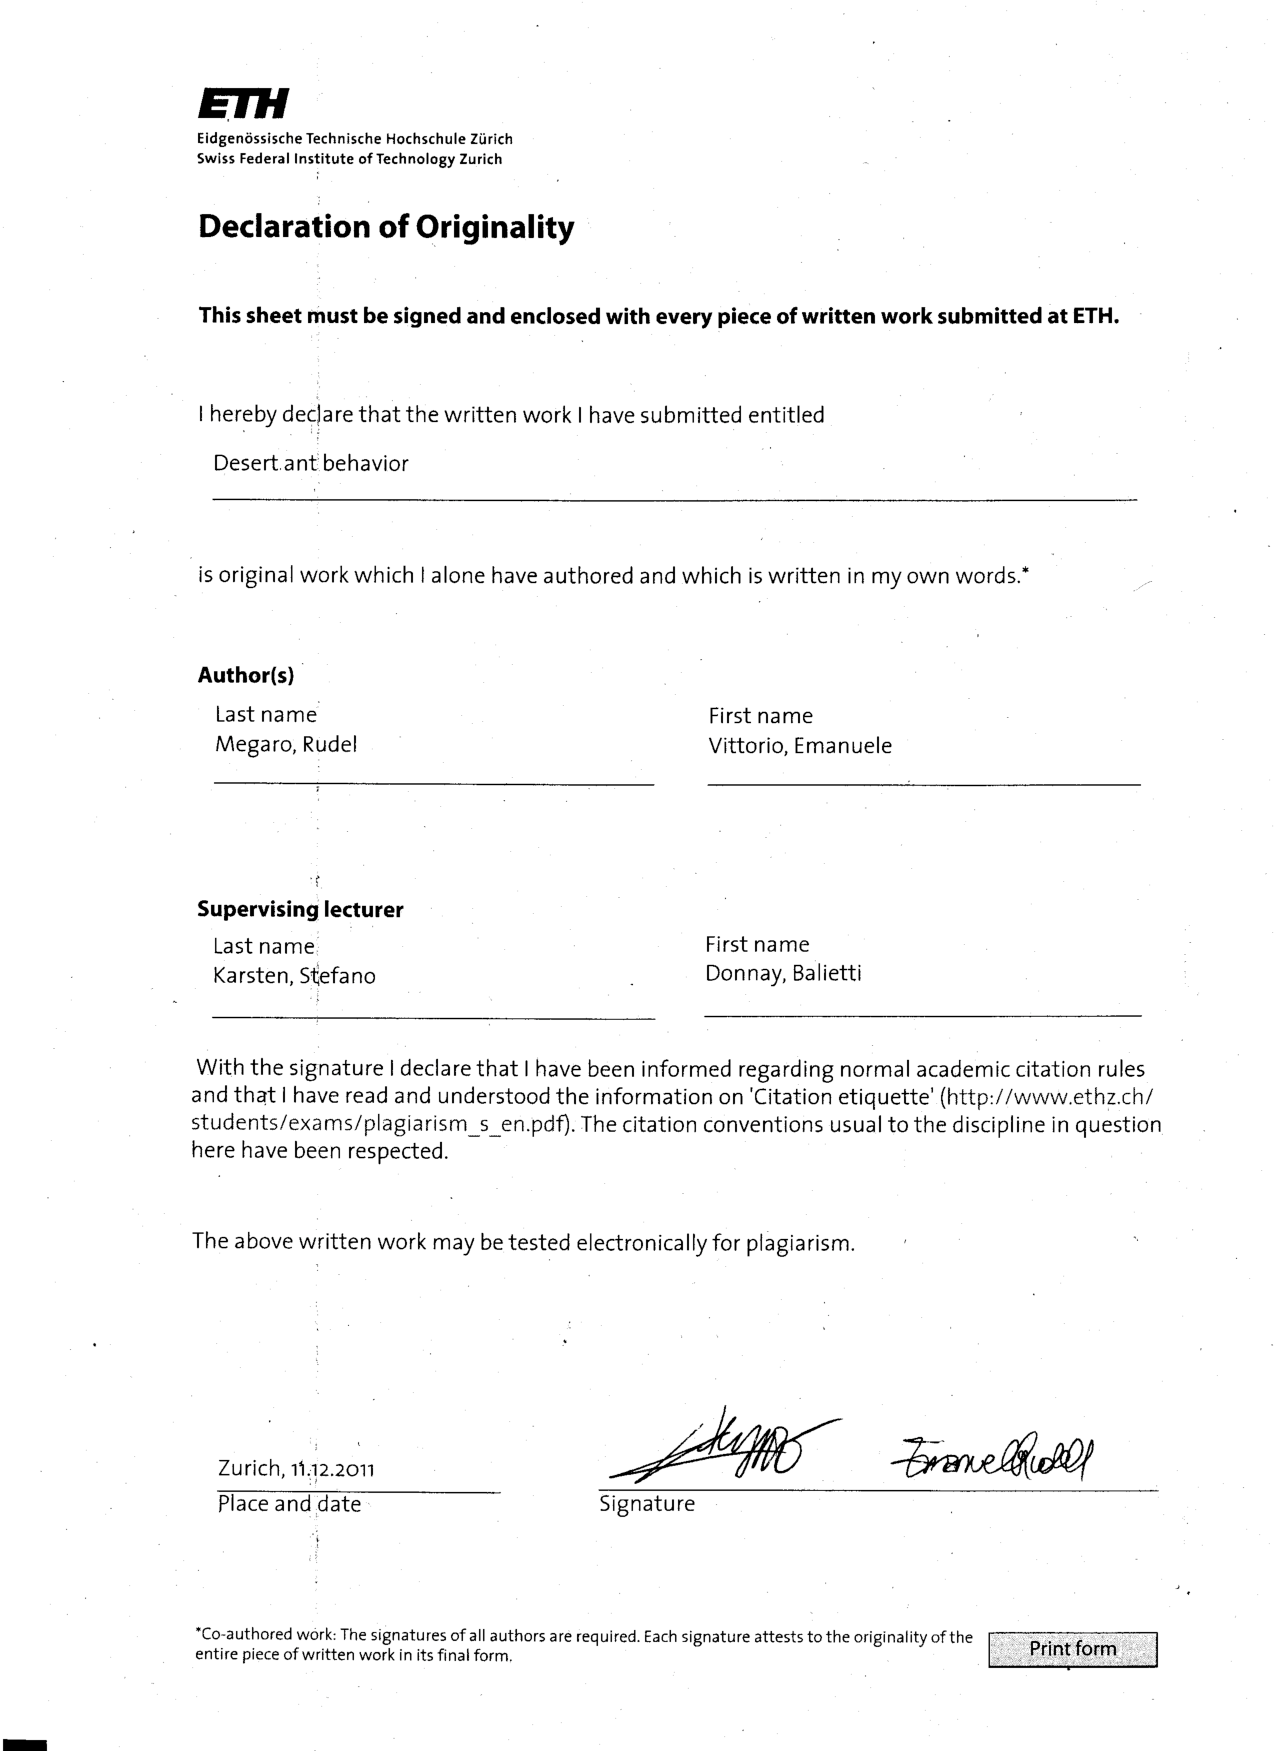
\includepdf[pages={1}]{plagiarism.pdf}


%%%%%%%%%% Table of content %%%%%%%%%%%%%%%%%

\begin{abstract}
In this article we present three different simulations of strategies adopted by ants to find a food source and to consequently return to their nest. The former strategy is based on pheromone trails and is the most common among ants, while the second and the third strategy --- called path and landmark integration, respectively --- are typically adopted by desert ants for a number of reasons to become throughout this paper. As a conclusion we also show a comparison between our simulations and the results obtained performing tests on actual ants.
\end{abstract}

\newpage

\tableofcontents

\newpage

%%%%%%%%%%%%%%%%%%%%%%%%%%%%%%%%%%%%%%%

\section{Individual contributions}
All the simulations and scripts for comparing the results have been implemented in pair. This choice allowed us to shape the design of the system together and to catch each other's mistakes very quickly. Moreover, the benefits of pair programming are that we both acquired knowledge of the complete program and one peer could help the other when stuck on a specific problem.

We split the task of writing the report so that one person would write a section and have the other to correct it afterwards --- and vice versa.

For the hash table class we implemented a simplified version of the one freely available at the MATALB central website\footnote{MATLAB central, Simple hashtable: http://www.mathworks.com/matlabcentral/fileexchange/6514}

\section{Introduction and Motivations}

Where are we now? It may seem a ridiculously easy question to ask ourselves, especially nowadays with the advent of GPS devices that can tell us our exact position no matter where we are. If we think about it, however, men have always used several reference systems in order to determine their location such as maps, streets, numbers and even stars and constellations. These information are conventionally defined and allow us, aside from being aware of where we are, to be share our position with others whatever the reason might be. Ok, so we know where we are.

How do ants know where they are? They sure don't have the technology that humans have developed and they don't have maps or streets or numbers either. Ants are actually pretty simple animals in terms of intelligence: a colony of 40'000 ants has approximately the same number of brain cells as a single human brain. It is thus ruled out the possibility that ants have a complex orientation system.

Despite being fairly simple insects, ants are one of the most fascinating creatures alive; they appeared on Earth about 130 million years ago and they're present pretty much anywhere in the world. The ant's population is estimated to be one quadrillion (a one followed by fifteen zeros) and they account for roughly 15\%-25\% of the total animal biomass. An ant can lift 20 times its own body weight and can cover a distance from its nest up to 200 meters. This last fact is really interesting in light of our previous question if we consider that it would correspond, keeping the same size-distance proportion, to a walk of about 35 kilometers for a human being. It is therefore of extreme interest to understand how ants can cover such a long distance without getting lost, and that is what we will try to do in the next section.

\section{Description of the Model}

\subsection{Pheromone-based orientation}
\subsubsection{Introduction}
When ants set out to leave their nest and start searching for a food source, they constantly emit a chemical called pheromone during their walk. The trail of chemical is useful as it allows ants to find their way back to the nest and it also tells the other ants --- since they can smell pheromones --- where a peer has been traveling. Whenever an ant finds a food source, it releases a larger amount of pheromones as it runs back to the nest as fast as it can. It is important to point out that pheromone is a chemical that evaporates quickly and it is thus essential that an ant marks a reliable path (i.e. one path that takes to a food source) with a stronger signal. As soon as other members of the colony notice the strong pheromone trail, they start following the path and release the same pheromone to keep the path marked. The advantage of the pheromone evaporating quickly is that when a food source is exhausted ants stop leaving pheromones on that exact path --- which becomes thus abandoned --- and start looking for the next provisions supplier without having to worry of ending up on an old trail.

% Figure 1
\begin{figure}[h!]
  \centering
    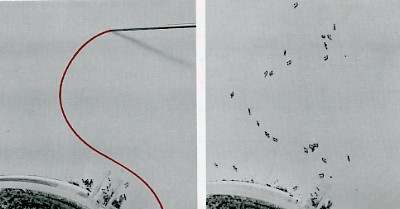
\includegraphics[width=.7\textwidth]{images/TrailPheromone.jpg}
     \caption{Ants follow an artificial pheromone trail (http://users.rcn.com/jkimball.ma.ultranet/BiologyPages/P/Pheromones.html).}
\end{figure}

\subsubsection{Pheromone modeling}
As stated above, pheromone is a chemical that evaporates fairly quickly. More precisely, its intensity decays exponentially in time as described in the formula
\begin{center}
$I(t)=I(t-\Delta t)*exp((log(\frac{1}{2})/t_c)\Delta t)$
\end{center}
(see reference [1])
where $t_c$ represents the characteristic evaporation time of the pheromone in a particular environment.

In our simulations the intensity of the pheromone will be represented by the following color map:

\begin{figure}[h!]
	\centering
    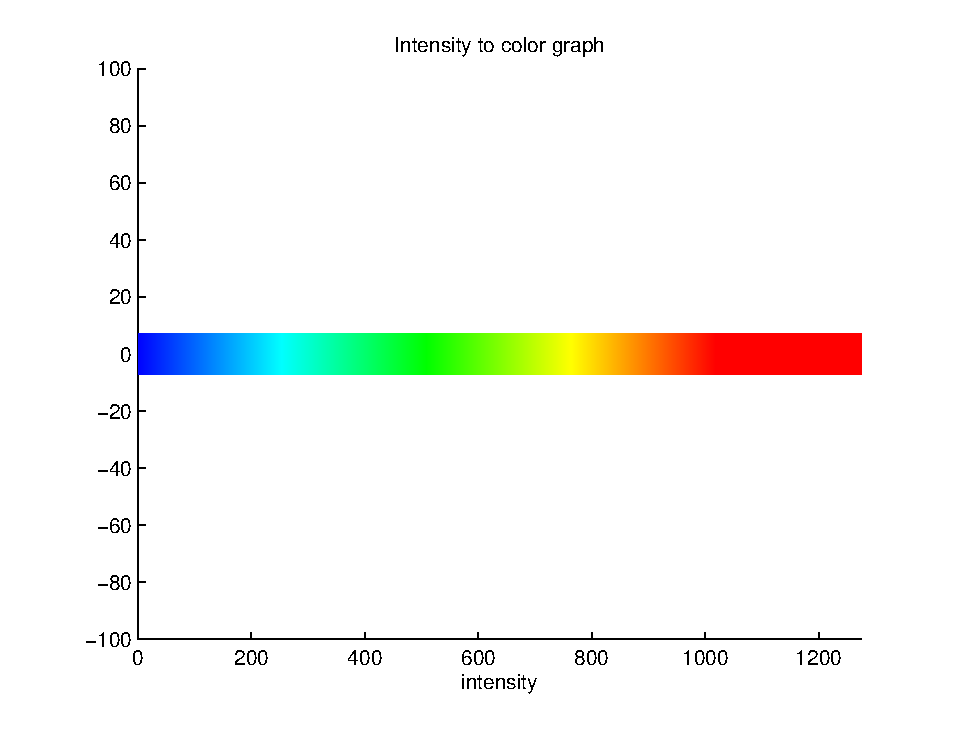
\includegraphics[width=.7\textwidth]{../sources/results/intensity2color.eps}
     \caption{The color associated to the pheromone's intensity.}
\end{figure}

Using the available experiments (see reference [2]) we have determined the evaporation time to be around 2 minutes in a very hot environment such as the Sahara desert. We chose this evaporation time because we want to find an answer to the following question:
\begin{center}
\emph{Which method, out of the three described in this article, is more suitable for desert ants (Cataglyphis fortis)?}
\end{center}

The pheromone decay is one variable to take into account for this first simulation, although the most important issue is the strategy adopted by ants to find a food source.

\subsubsection{Strategy}
As they leave the nest, ants do not have an effective strategy for finding food: they just start walking randomly with the hope of running into a food supply. However, they always make sure not to walk too far away from the nest: if the search is unsuccessful for a given distance, they turn back to the nest direction and start walking in a different one. Since the walk's length cannot be computed relying just on pheromone trails it is deducible that ants must have a complementary mean to keep track of the distance from the nest. This method is called path integration and is the subject of the next subsection.

\subsection{Path integration}

Similar to techniques used by men in the past centuries to find out their current position, ants can estimate their location advancing of a small step from a previously computed estimation based upon known measures such as the number of steps walked in a fixed amount of time. As observed in \emph{Path integration in desert ants, Cataglyphis fortis} by M\"{u}ller and Wehner, path integration has a great advantage over pheromone trails:
\begin{center}
	\begin{quotation}
		``Path integration means that the animal is able to continuously compute its present location from its past trajectory and, as
		a consequence, to return to the starting point by choosing the direct route rather than retracing its outbound trajectory.''
	\end{quotation}
\end{center}

At a time step $n$, an ant computes
\begin{enumerate}
\item the distance $l_n$ that separates the ant from the nest to its current location
\item the angle $\phi_n$ the ant needs to turn to (with respect to its current position) to point towards the nest
\end{enumerate}

using the following formulas

\begin{center}
$\phi_{n+1} = \phi_n + k*\frac{(180^{\circ} - \delta)(180^{\circ} + \delta) \delta}{l_n}$
\end{center}
\begin{center}
$l_{n+1} = l_n + 1 - \frac{\delta}{90^{\circ}}$
\end{center}

where $k$ is the fitting constant and $1$ is the unit length walked at each step. These formulas have been derived from the results of several tests on desert ants, which have showed that ants are not able to solve the problem of path integration correctly most likely because of their limited brain functions. $\phi_n$ and $l_n$ are always pointing to the nest and together they form what is called the \textbf{global vector}.

The drawback of path integration is that being an estimated computation it inherently has an approximation error that grows with time. In extreme cases the ant might even walk home in a completely different direction from the actual one because of sharp turns causing large approximation errors of the angle $\phi_n$. If that's the case, the ant usually walks the whole distance $l_n$ in the direction that it believes to be correct and then, not finding the nest, will start searching for it in the neighborhood with a random walk.

\subsection{Landmark orientation}

Landmark orientation is a technique used in conjunction with path integration: desert ants take a snapshot of the surrounding environment and match it with a well known place or object like the nest, the food source or an obstacle encountered on a walk. Since it is not explained, or probably not even known, how exactly ants match the landmarks, and we will make some assumptions of how they solve this problem in the implementation section. In that paper (see reference [3]), the only landmarks used are four black cylinders surrounding the ants' nest. Two interesting (and mutually exclusive) hypothesis have thus been formulated and verified:
\begin{enumerate}
\item the global vector is reset as soon as the ant recognizes the landmark array
\item the global vector is not reset when the ant sees the landmark array
\end{enumerate}

A way to find out which hypothesis is correct is to conduct the following four-phases test:
\begin{description}
\item[Phase 1] ants starts foraging in an environment where the four cylinders are placed around the nest, as depicted in the figure below.
% Figure 2
\begin{figure}[h!]
  \centering
    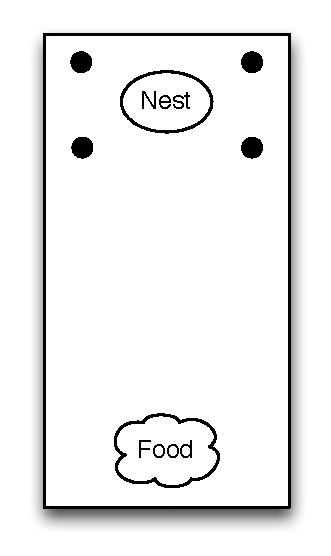
\includegraphics[width=.25\textwidth]{images/phase1}
     \caption{The initial setup in phase 1.}
\end{figure}
\item[Phase 2] After about 30 foraging runs and when the ants arrive at the food source, they are displaced in a different area with no nest and landmarks. The ants start following their global vector recorded using path integration, but when the global vector is zero and yet there's no trace of the nest, the ants start looking around in a circular fashion.
\item[Phase 3] The four landmarks are now restored in a fictitious position --- i.e. where once again, there's no nest --- and when the ants see (or perceive) the landmarks they start walking towards them. It is not clear how exactly ants handle the landmark recognition, thus we will make some assumptions when implementing this behavior in the next section.
% Figure 3
\begin{figure}[h!]
  \centering
    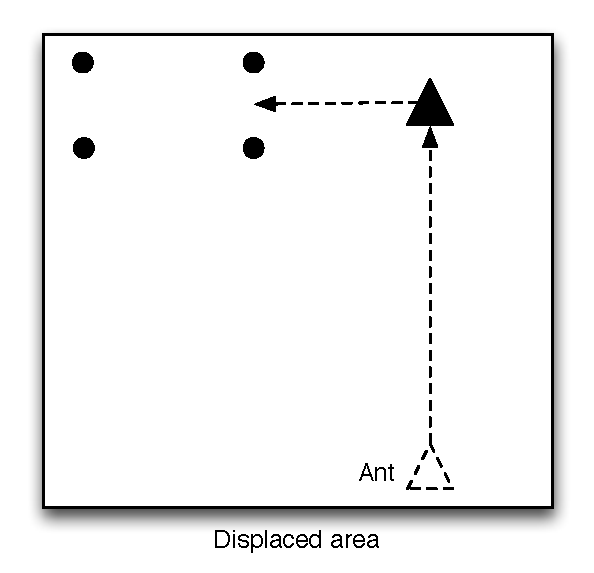
\includegraphics[width=.5\textwidth]{images/phase3}
     \caption{The ant does not find the nest when its global vector is zero. As it notices the new landmarks, it starts walking towards them.}
\end{figure}
\item[Phase 4] The landmarks are successively removed. At this point, we can find out whether ants reset or not their global vector after having recognized the landmarks. If they did, they will keep looking for the nest right where they are, while if they didn't, they will follow the global vector until the original nest's position, and only at this point they'll start looking for the nest. The picture below shows the two possible scenarios.
% Figure 4
\begin{figure}[h!]
  \centering
    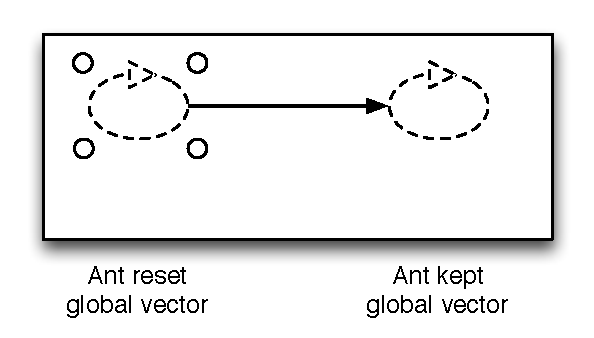
\includegraphics[width=.6\textwidth]{images/phase4}
     \caption{The ant goes back to where it thinks the nest is, according to its global vector.}
\end{figure}
\end{description}

The test carried out by Knaden and Wehner showed that ants actually never reset their global vector, instead they keep it as a backup in case the landmark recognition fails. In our simulation we will make use of this fact and compare our results with the ones obtained testing actual desert ants.

\section{Implementation}

\subsection{General implementation}
The three simulations all take place on the same continuous two dimensional space defined as \textbf{ground}, where ants can freely move within the boundaries. The ground keeps track of the nest and food source locations, as well as the landmarks, the ants moving on it and the pheromone particles they have released on the ground.

\subsubsection {Ants' random walk}
As we previously mentioned that ants walk randomly to find a food source, we also observed that they never venture too far away from their nest. Additionally, ants rarely perform sharp turns and because of these two reasons implementing a simple random walk would have not produced a realistic simulation of how actual ants solve the task of finding a food source. We thus opted for a random walk with the following constraints:

\begin{itemize}
\item at each time step, the ant will change its direction of an angle chosen from a normal random distribution. This constraint makes sure that the ant will not abruptly change direction.
\item the mean of the normal distribution for the angle is based on a weighted distance from the nest location, which we assume the ant can estimate thanks to path integration. Put it simple, the farther the ant walks, the greater is the probability that it will eventually turn around and start walking in another direction.
\end{itemize}

This pseudocode represents the random walk implemented for the Ant class:

\lstinputlisting[language=Eiffel]{pseudocode/randomwalk.e}

Furthermore, at each time step the ant keeps updating its global vector, releasing pheromone particles --- whose intensity changes depending on whether it is walking randomly or following a well known trail --- and looking for possible landmarks, although it will only make use of them in the third simulation.

\subsection{Pheromone-based orientation}

One of the fundamental questions that we asked ourselves at the beginning of this research was
\begin{center}
	\emph{How do ants communicate to each other useful information such as the directions to a food source?}
\end{center}
With this first simulation we would like to observe that ants communicate using pheromones of varying intensity to provide useful information to their peers.

We thus let an arbitrary number of ants start looking for a food source. The ants walk randomly trying to find a food source (also known as foraging) and release pheromone particles of a mild intensity in order to be able to find their way back to the nest --- even though they will actually make use of path integration for the latter task.

The simulations are saved as video files which will be compared in the next section with still images of different papers that performed experiments on real ants.

\subsection{Path integration}

The purpose of this simulation is to assess the error accumulated over time using the formulas for path integration described in the previous section. The simulation is based on the same experiments conducted by M\"{u}ller and Wehner (see reference [4]):

\begin{enumerate}
\item An ant walks into a pre-established path that consists of two arms of different lengths.
\item Past the second arm, the ant will head back to the nest through a direct route. The angle between the two arms changes between each run to observe how the path integration error is influenced by the sharpness of one turn.
\end{enumerate}

\subsection{Landmark orientation}

The third simulation shows ants behavior when an array of landmarks is placed around the nest. We will skip the learning process since the goal is to observe the fact that ants do not reset their global vector in presence of landmarks. The simulation consists of the following steps:

\begin{enumerate}
\item the ant is initially in the displaced area (phase 2) and starts walking following its global vector. When it realizes that the nest is not where it should be anymore, the ant starts walking randomly searching for the nest. This phase lasts two minutes.
\item For one minute the four landmarks are placed in a fictitious position. If the ant is close enough to somehow perceive the landmarks, it will start looking for the nest inside the area defined by those four landmarks.
\item The landmarks are removed and the ant is free to move in the area for another five minutes. We will observe that it will first return to where the ant thinks the nest should be, and only after making sure that the nest is most certainly in that position, it will (randomly) start searching for the nest once again.
\end{enumerate}

Regarding how ants recognize landmarks, we made the following assumptions:
\begin{itemize}
\item if ants can only see one landmark, they start walking towards to it;
\item if ants can see two landmarks, they approximately walk between the two, and
\item if ants recognize three or more landmarks, they will estimate the middle point between them and walk in that direction.
\end{itemize}

One problem we had to deal with in the implementation of this simulation is that our artificial ant must be able to decide in which direction it should go after two landmarks have been detected. Of course a real ant doesn't need to tackle such a problem because it knows the direction it came from and thus the direction it has to follow is trivial. Artificial ants, on the other hand, do not keep track of their previous locations and the figure below depicts the problem that could arise:

% Figure 5
\begin{figure}[h!]
  \centering
    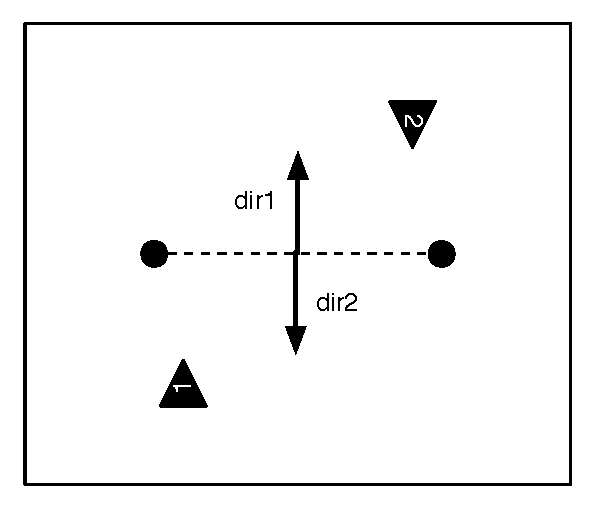
\includegraphics[width=.6\textwidth]{images/ambiguous_direction}
     \caption{The artificial ant needs to compute the direction in which it should walk. For both artificial and real ants, however, the point of view from 1 and 2 is indistinguishable.}
\end{figure}

The solution is to project the coordinates --- y-coordinates in the picture --- on the dashed line between the two landmarks (as shown below) and depending on whether the projected coordinates are smaller or bigger than the original values, we set the ant's direction to point downwards or upwards, respectively.
\newpage
\section{Simulation Results and Discussion}

\subsection{Pheromone-based orientation}
The obtained videos of different runs of the simulation clearly showed that there's a strong cooperation between ants belonging to the same nest. As soon as one of them discovers a reliable food source, it increases the pheromone's intensity to alert its peers that the path on which it is moving leads to a food source. This fact is in accordance with the papers that describe the pheromone-based orientation (see references), but unfortunately they did not provide pictures or videos of an actual ants' cooperation. The number of foraging ants was limited to a maximum of 7 for computational limit reasons; in reality a much bigger number of ants is employed to find a food source.

\begin{figure}
\centering
\begin{tabular}{c}
	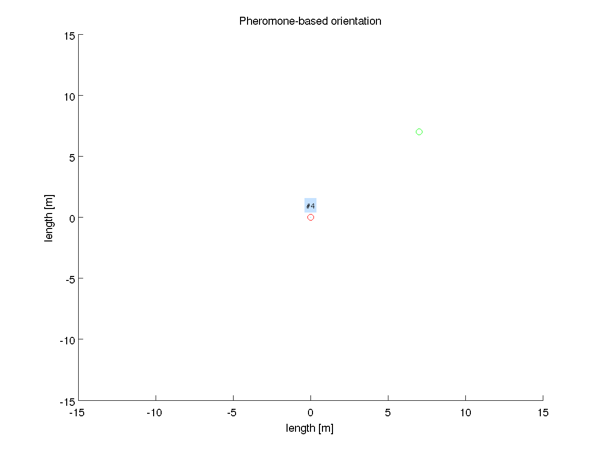
\includegraphics[width=.9\textwidth]{../sources/results/pheromoneResults/snap_0001.png} \\
	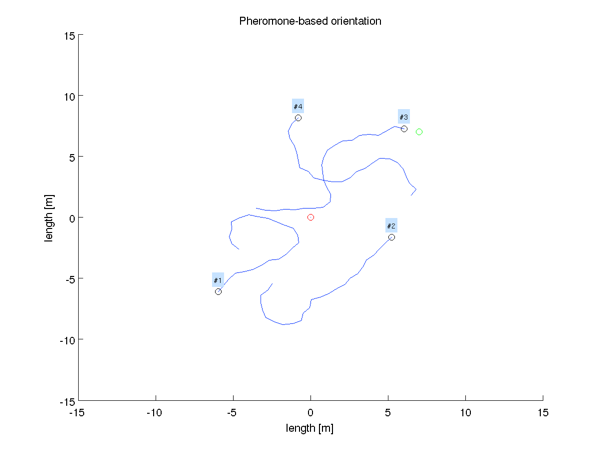
\includegraphics[width=.9\textwidth]{../sources/results/pheromoneResults/snap_0036.png}
\end{tabular}
\caption{Above: four ants depart from the nest (red circle) and start looking for a food source (green circle). Below: random walk of the four ants.}
\end{figure}
\begin{figure}
\centering
\begin{tabular}{c}
	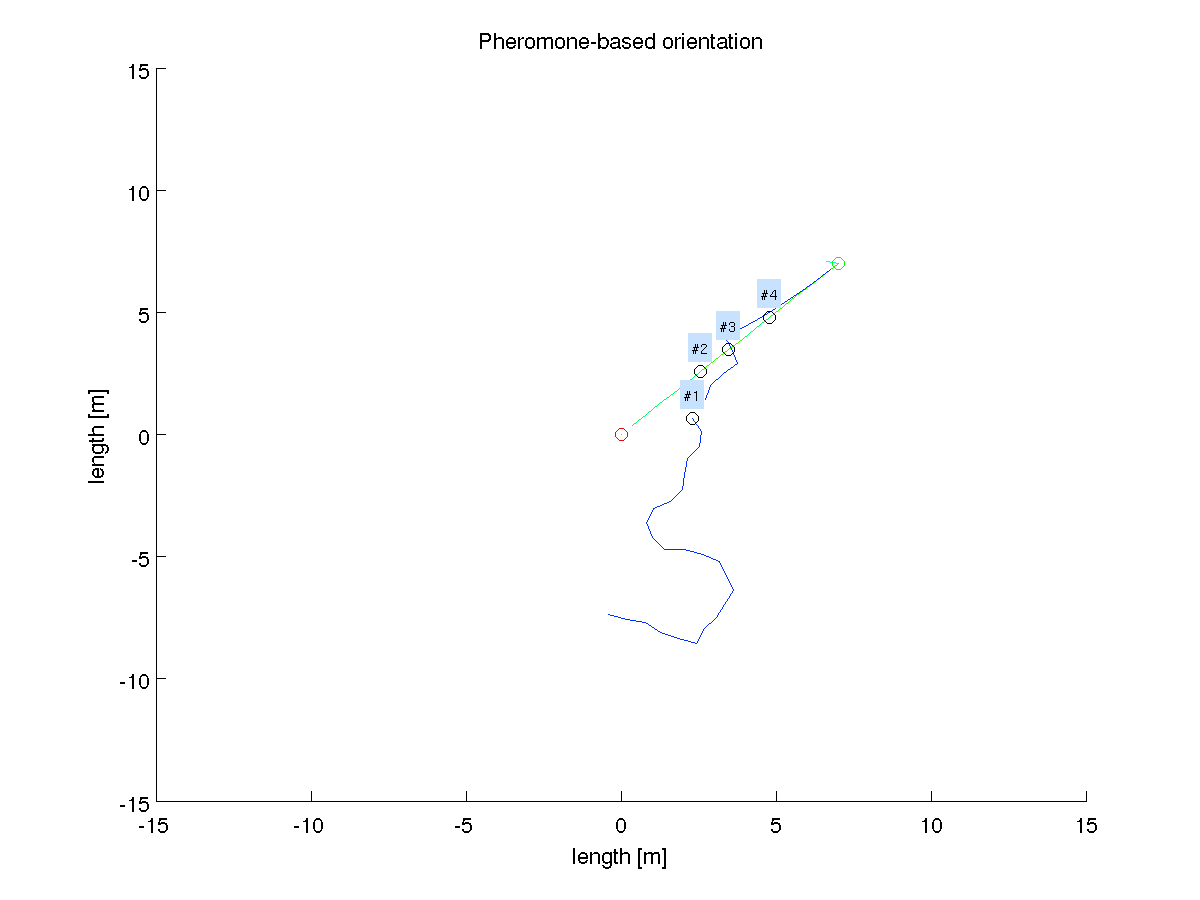
\includegraphics[width=.9\textwidth]{../sources/results/pheromoneResults/snap_0097.png} \\
	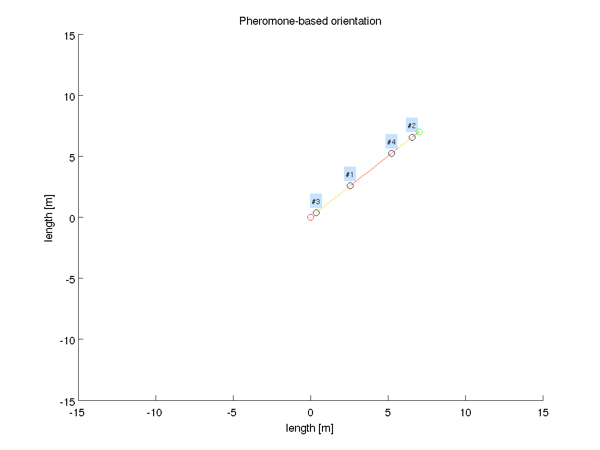
\includegraphics[width=.9\textwidth]{../sources/results/pheromoneResults/snap_0154.png}
\end{tabular}
\caption{Above: one ant has found a food source and its peers, smelling the pheromone, walk along that path. Below: all the ants are now walking on the path that connects the nest to the food source.}
\end{figure}
In the figures above, the color of the pheromone track left by ants changes depending on the intensity (blue represents low intensity, while red represent a high intensity).

We also show a plot of the pheromone's decay in the Sahara desert. This graph gives us an idea of how fast the pheromone track left by a desert ant disappear.
\begin{figure}[h!]
	\centering
	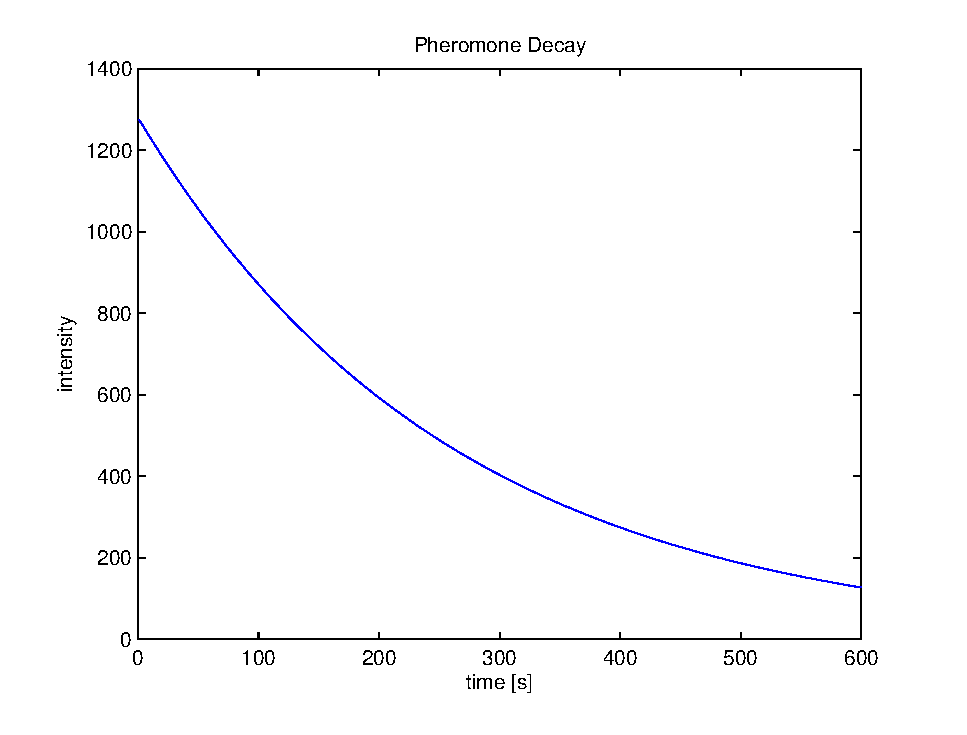
\includegraphics[width=.8\textwidth]{../sources/results/pheromoneDecay.eps}
	\caption{Pheromone decay in the Sahara desert.}
\end{figure}

It is important to point out that in hostile environments such as the Sahara desert, the pheromone evaporates so quickly that ants would only have a very limited amount of time (a couple of minutes) to venture out of the nest and make return before they lost track of their own pheromone and get lost. In the next section we will explain why this does not happen in reality.

\subsection{Path integration}
The simulation ran for the path integration model was the same as the test conducted in [4]. Our test yielded a graph which has the same trend as the reference paper, but whose values are in strong disagreement. Comparing the differences between the results of the paper and our simulations, the error angle (in degrees) measured in our simulation resulted at least twice as big as the original one.

\begin{figure}[h!]
	\centering
	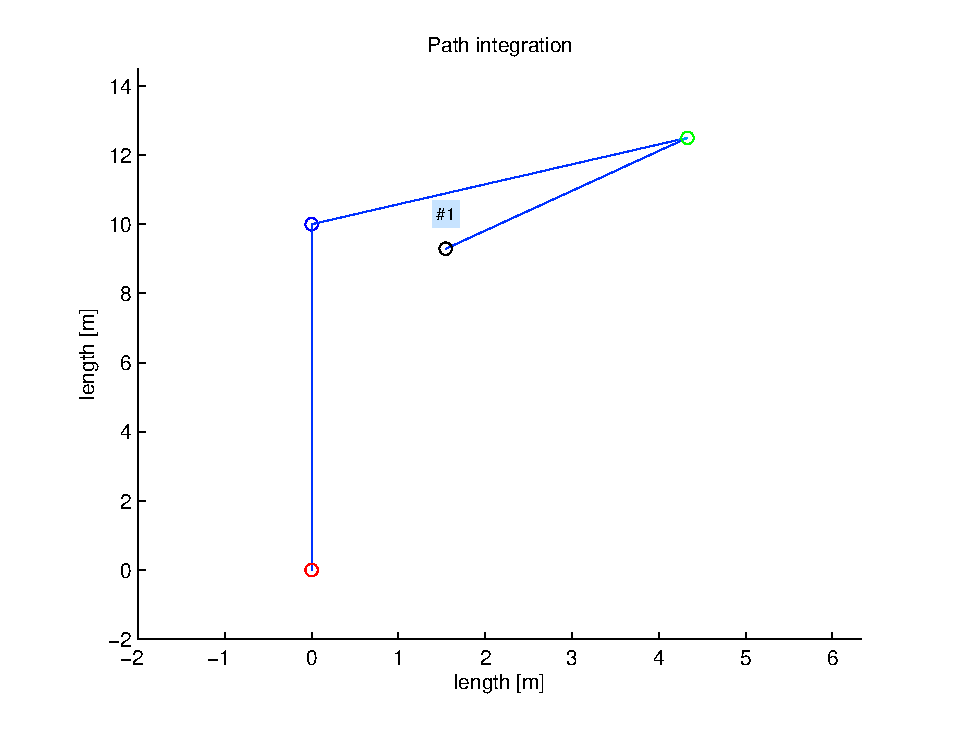
\includegraphics[width=.8\textwidth]{../sources/results/pathIntegrationResults/animation.eps}
	\caption{The ant, marked as ``\#1'', should return to the nest (red circle) after it left the food source (green circle). However, the angle computed with the formulas for path integration is not computed correctly.}
\end{figure}

We could not find out the reason of this strange behavior; even changing the fitting constant in the formula for computing $\phi_n$ did not help the simulation to improve. It is very likely that the bug resides somewhere in our code, yet we were not able to catch it before handing in this paper. In the other two simulations we therefore haven't used this particular implementation of path integration.

\subsection{Landmark orientation}
The test described in the third section has been simulated once using the same locations as in the original paper (see [3]) and once using a different location for the fictitious nest and rotating the landmarks. This procedure ensured that our implementation worked in different situations. Both the results of the first and second simulation match the ones in the original paper (except for the coordinates of the second test, of course) as shown below:
\begin{figure}[h!]
	\centering
	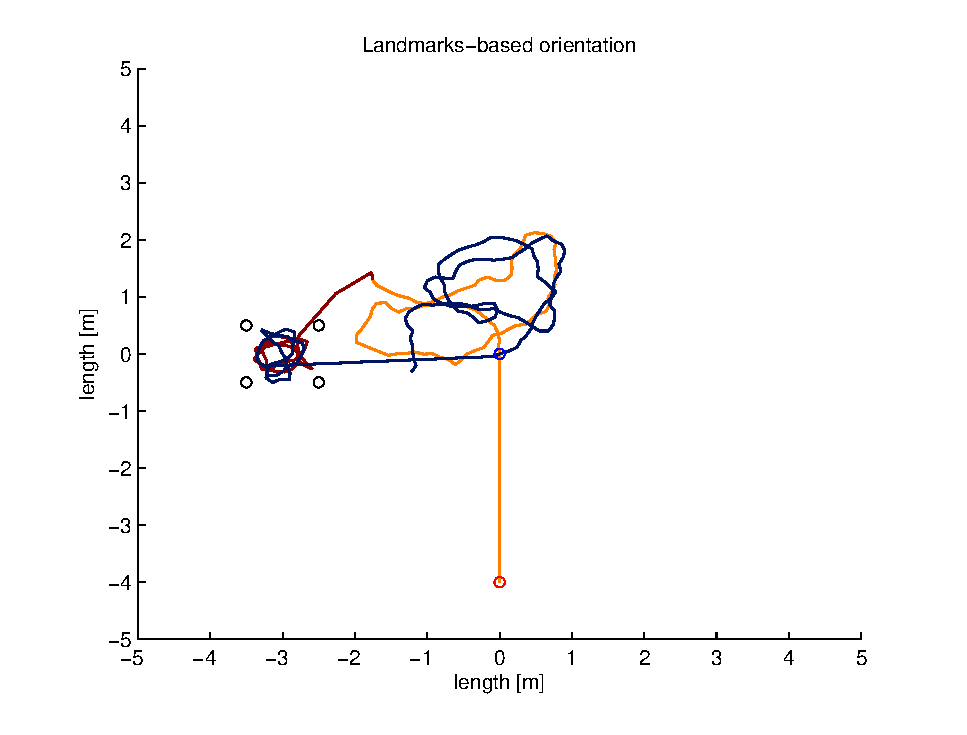
\includegraphics[width=.8\textwidth]{../sources/results/fourLandmarksResults/fourLandmarks.eps}
	\caption{The first test is the same as the one in [3]. The circle on the bottom represents the location at which the ant was released; the circles on the left represent the landmarks; the different colors of the ant's path, namely orange, dark red and blue represent the three phases (return to the nest, landmarks placed, landmarks removed). The blue circle in the middle represents the original position of the nest.}
\end{figure}
\begin{figure}[htbp!]
	\centering
	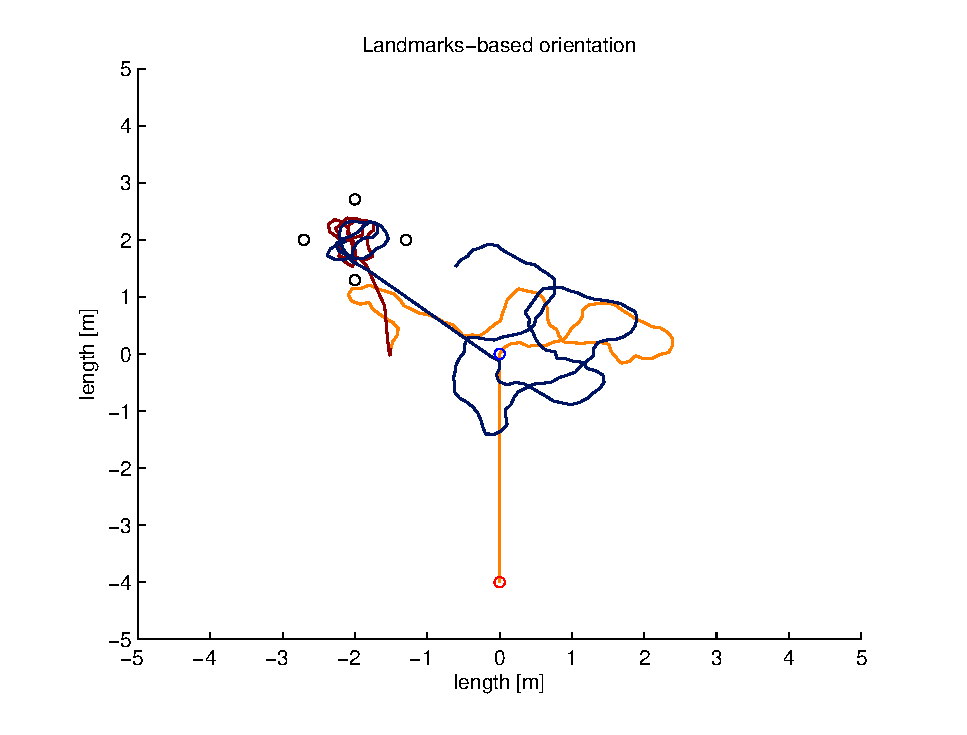
\includegraphics[width=.8\textwidth]{../sources/results/fourLandmarksResults/fourLandmarksRotated.eps}
	\caption{This test is similar to the one above, except for the fact that the landmarks have been placed higher with respect to the original position of the nest and it has also been rotated.}
\end{figure}
We found really interesting the fact that a random walk (slightly constrained as explained above) closely represents how ants actually perform a search for their nest. The relatively simple structure of the ant's brain could justify the lack of a more elaborated strategy. On a different paper\footnote{\emph{The hidden spiral: systematic search and path integration in desert ants, Cataglyphis fortis}, M. M\"{u}ller and R. Wehner, http://www.springerlink.com/content/l21217t6pw686314/} is observed that desert ants perform a search for the nest in a spiral course around the point where the ant believed the nest was at.
\newpage
\section{Summary and Outlook}

In this section we would like to answer the questions we had asked ourselves at the beginning of this research and those who later arose when developing the models and implementations.

\begin{center}
	\emph{Which method, out of the three described in this article, is more suitable for desert ants (Cataglyphis fortis)?}
\end{center}
It should be clear by now that it is impossible for desert ants to only use a pheromone-based orientation: if they couldn't find any food within a few minutes they would get lost looking for their way back to the nest. Nevertheless, the desert ants' nest emits a strong signal of pheromones and makes it easy for ants in the close neighborhood to find the nest entrance.

Since the desert lacks of landmarks and is continuously changing because of storms, desert ants cannot use landmark orientation either as their primary navigation system.

Desert ants thus mainly rely on path integration to navigate and they also make use of skylight information (not handled in this paper).

\begin{center}
	\emph{Are the three methods described independent of each other?}
\end{center}

The pheromone-based orientation is independent of the other two techniques, yet it is never used alone. Ants take a safe approach and always use a combination of the different orientation systems.

\begin{center}
	\emph{Do ants communicate their position and other information to help each other?}
\end{center}

Ants do not communicate directly with each other. They indirectly transmit information regarding the position of a food source using pheromones, but they do not share any other information.

\begin{center}
	\emph{How can ants remember exactly a path that is thousands of times their own body length?}
\end{center}

They don't. An old conjecture assumed that ants could retrace their way back to the nest by reversing the order and direction in which they previously took their steps. This mechanism is simply not applicable to ants as it would require the insect to store an enormous amount of information. Since ants have a very small brain, this conjecture can be easily rejected.

%TODO: write conclusion? further work: add mixed techniques
The work conducted fully answered to our questions, and in particular it showed that when studying ants behavior there is no clear distinction between the usage of the different techniques. All of the three are indeed often combined together to achieve the best outcome possible. As a future work it would be therefore interesting to be able to combine the three methods and train the ants on a more complex environment. The unexpected results of the path integration did not allow us to perform perfectly realistic simulations and they will need further investigation to find the cause that lead to a large estimation error of the angle.

\section{References}

\begin{tabular}{ c p{14cm}}
  $[1]$ & \emph{Alice in Pheromone Land: An experimental Setup for the Study of Ant-like Robots}, S. Garnier, F. T\^{a}che, M. Combe, A. Grimal and G. Theraulaz, 2007 \\
  $[2]$& \emph{Pheromone trail decay rates on different substrates in the Pharaoh's ant, Monomorium pharaonis}, R. Jeanson, F. Ratnieks and J. Deneubourg, 2003  \\
  $[3$] & \emph{Nest mark orientation in desert ants Cataglyphis: what does it do to the path integrator?}, M. Knaden and R. Wehner, 2005  \\
  $[4]$ & \emph{Path integration in desert ants, Cataglyphis fortis}, M. M\"{u}ller and R. Wehner, 1998  \\
\end{tabular}

\newpage

\appendix
\section{Matlab code}
\subsection{Ant.m}
\lstinputlisting[language=Matlab, morekeywords={classdef,methods,properties}]{../sources/Ant.m}

\subsection{Ground.m}
\lstinputlisting[language=Matlab, morekeywords={classdef,methods,properties}]{../sources/Ground.m}

\subsection{intensity2color.m}
\lstinputlisting[language=Matlab, morekeywords={classdef,methods,properties}]{../sources/intensity2color.m}

\subsection{Hashtable.m}
\lstinputlisting[language=Matlab, morekeywords={classdef,methods,properties}]{../sources/Hashtable.m}

\subsection{pheromoneAnimation.m}
\lstinputlisting[language=Matlab, morekeywords={classdef,methods,properties}]{../sources/pheromoneAnimation.m}

\subsection{PheromoneParticle.m}
\lstinputlisting[language=Matlab, morekeywords={classdef,methods,properties}]{../sources/PheromoneParticle.m}

\subsection{projectPointOnLine.m}
\lstinputlisting[language=Matlab, morekeywords={classdef,methods,properties}]{../sources/projectPointOnLine.m}

\subsection{randomWalkTest.m}
\lstinputlisting[language=Matlab, morekeywords={classdef,methods,properties}]{../sources/randomWalkTest.m}

\subsection{twoArmGlobalVectorAnimation.m}
\lstinputlisting[language=Matlab, morekeywords={classdef,methods,properties}]{../sources/twoArmGlobalVectorAnimation.m}

\subsection{twoArmGlobalVectoTest.m}
\lstinputlisting[language=Matlab, morekeywords={classdef,methods,properties}]{../sources/twoArmGlobalVectorTest.m}

\subsection{updateGround.m}
\lstinputlisting[language=Matlab, morekeywords={classdef,methods,properties}]{../sources/updateGround.m}

\subsection{vector2angle.m}
\lstinputlisting[language=Matlab, morekeywords={classdef,methods,properties}]{../sources/vector2angle.m}

\end{document}  



 
